\documentclass[10pt,a4paper]{article}

\usepackage[margin=0.75cm]{geometry}
\usepackage[utf8]{inputenc}

\usepackage{amsmath}
\usepackage{amssymb}
\usepackage{biblatex}
\usepackage{textcomp}
\usepackage{gensymb}
\usepackage{paracol}
\usepackage{parskip}
\usepackage{tikz}
\usepackage{titlesec}
\usepackage{verbatim}
\usepackage{xcolor}

\titleformat{\section}[block]{\Large\bfseries\filcenter\color{black}}{\thesection}{1em}{}
\titleformat{\subsection}[block]{\bfseries\filcenter\color{black}}{\thesubsection}{1em}{}

\setlength{\columnsep}{25pt}

\tikzset{
    rounded-box/.style = {draw=teal, fill=white, thin, rectangle, rounded corners, inner sep=5pt, inner ysep=10pt},
    rounded-box-title/.style = {fill=teal, text=white, font=\bfseries},
}

\addbibresource{references.bib}

\begin{document}
\title{Discrete Mathematics}

\section{Methods of Proof}

\begin{itemize}
    \item A \textbf{direct proof} proceeds by establishing a chain of implications $P \Rightarrow P_1 \Rightarrow \dots \Rightarrow P_n \Rightarrow Q$ leading directly from $P$ to $Q$. \\

    \item A \textbf{proof by contradiction} assumes that the hypothesis $P$ is true, just as in a direct proof, but then supposes that the conclusion $Q$ is false. \\

    \item Closely related to the method of proof by contradiction is \textbf{proof by contrapositive}: The negative of a statement $P$ is the statement "it is not the case that $P$", abbreviated symbolically as $\neg P$ and pronounced "not $P$".
\end{itemize}

\subsection{Mathematical Induction}

\begin{paracol}{2}

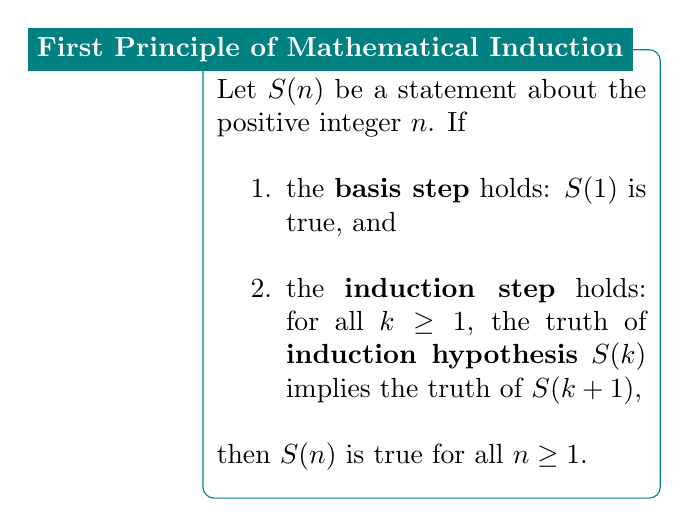
\begin{tikzpicture}
\node [rounded-box] (box){\begin{minipage}{0.45\textwidth}
    Let $S(n)$ be a statement about the positive integer $n$. If \\

    \begin{enumerate}
        \item the \textbf{basis step} holds: $S(1)$ is true, and \\
        \item the \textbf{induction step} holds: for all $k \geq 1$, the truth of \textbf{induction hypothesis} $S(k)$ implies the truth of $S(k+1)$, \\
    \end{enumerate}

    then $S(n)$ is true for all $n \geq 1$.
\end{minipage}};
\node[rounded-box-title, left=10pt] at (box.north east) {First Principle of Mathematical Induction};
\end{tikzpicture}

\switchcolumn

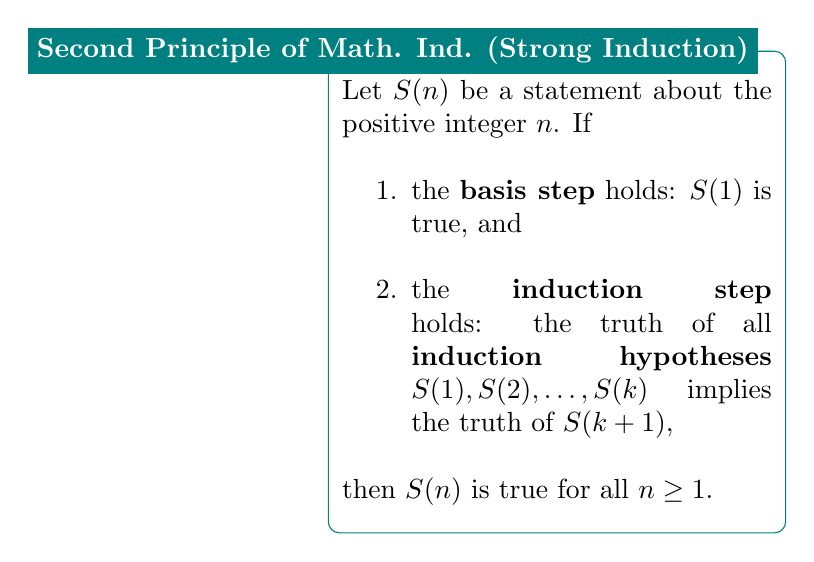
\begin{tikzpicture}
\node [rounded-box] (box){\begin{minipage}{0.45\textwidth}
    Let $S(n)$ be a statement about the positive integer $n$. If \\

    \begin{enumerate}
        \item the \textbf{basis step} holds: $S(1)$ is true, and \\
        \item the \textbf{induction step} holds: the truth of all \textbf{induction hypotheses} $S(1), S(2), \dots, S(k)$ implies the truth of $S(k+1)$, \\
    \end{enumerate}

    then $S(n)$ is true for all $n \geq 1$.
\end{minipage}};
\node[rounded-box-title, left=10pt] at (box.north east) {Second Principle of Math. Ind. (Strong Induction)};
\end{tikzpicture}

\end{paracol}

\input{section-2-combinatorics} \newpage
\input{section-3-asymptotics} \newpage
\section{Graphs}

The adjacency matrix of a graph is always symmetric
(it is not necessarily the case when considering digraphs).

Adjacency matrices can be generalized to take values other than 0s and 1s,
which allows weighted graphs to be defined.

Weighted graphs are particularly useful when edges represent distances or delays between vertices,
because values in the adjacency matrix can be used to indicate the corresponding quantities.

A path is an ordered sequence of edges that are distinct from one other, and is obtained from
a sequence of vertices by joining any two consecutive vertices in the corresponding edge.

Paths are often confused with walks. A walk is a sequence of vertices, such that
any two consecutive vertices form an edge in the graph. The difference is that,
in a path, an edge cannot appear twice.

A cycle in a graph is a path in which the extremities are identical.

The length of a path is the length of the sequence of edges.
For weighted graphs, the length corresponds to the sum of the weights.

A graph is said to be connected if, for any two vertices there exists a path having these vertices as extremities.

Trees are connected graphs that are cycle-free.

Note that trees are often confused with rooted trees, in which connected vertices have a specific relationship with one another.
Rooted trees can be defined by choosing one arbitrary vertex to be the root of the tree.

A complete graph includes all possible edges.

What is the size of a complete graph with an order of $n$? $n (n-1) / 2$.

Representations:

In terms of graph adjacency matrices, arrays are effecient to check if two vertices $u$ and $v$ are
connected by an edge. On the other hand they are not that efficient if you want to retrieve all the
neighbours of $u$, because you need to test each vertex $v$ one by one.

(Linked) lists are not adjacent in memory.
If each vertex has only a few neighbours, representing only neighbors with lists can significantly save memory.
On the other hand, checking if $u$ and $v$ are connected by an edge may require you to search the full list of $u$'s neighbours.

Consider a data structure for which the number of elements has to be defined beforehand. Is it a list or a array? Array.

We store the adjacency matrix of a graph with an order of 20 in an array. How many elements does this array contain? $400$.

Dijkstra's algorithm (shortest paths in nonnegatively weighted graphs):
DFS and BFS can't be directly applied to find shortest paths in weighted graphs.
A BFS favours a smaller number of hops from the initial vertex, regardless of the weights.
Dijkstra's algorithm is a modification of the BFS that allows us to find shortest paths, even in the presence of weights, if those are non-negative.
The simplest way to describe Dijkstra's algorithm is to imagine the starting vertex as a tap from which water is pouring out. The water will progress along the vertices and traverse the graph with a speed inversely proportional to the edge weights, so it's going to reach the closest vertices first.
BFS explores vertices by increasing the hops from the starting vertex. Dijkstra's algorithm explores vertices by increasing the distance from the starting vertex.
BFS uses a queue as its queuing structure. Dijkstra's algorithm uses a min-heap as its queuing structure, and stores vertices as keys, and distances to the starting vertex as values.

A priority queue is an abstract data type where each element has a priority, and the element with the highest (or lowest) priority is dequeued first. It can be implemented using various data structures like arrays, linked lists, or heaps.
A min-heap is a specific implementation of a priority queue that uses a binary tree structure where the parent node is always smaller than or equal to its child nodes, ensuring the smallest element is at the root.

Dijkstra's Algorithm finds the shortest path by exploring all possible paths uniformly based on cumulative edge weights from the source node.
A* enhances Dijkstra's by incorporating a heuristic function that estimates the cost to reach the goal, prioritizing paths likely to lead to the destination faster.
Dijkstra's algorithm guarantees optimal solutions for graphs with non-negative edge weights. A* guarantees optimality if the heuristic is admissible (never overestimates the true cost).
Dijkstra's algorithm explores all possible paths uniformly, making it slower for large graphs. A* excels in pathfinding scenarios like navigation systems where there is a defined start and goal node.

The complexity of an algorithm is a measure of the maximum number of elementary operations that are needed for its execution, as a function of the size of the input.

The Travelling Salesman Problem (TSP) is a problem in which we aim to find the shortest route going through all vertices of a complete weighted graph from an initial vertex.

In computer science, a reduction is a method for transforming one problem into another problem, typically for which solutions are already known.
To better understand reduction, think of language translation. Imagine you have a way to solve a problem in French, but your problem is expressed in English. A possible solution is to first translate your problem into French, solving it in French, then translating the solution back to English. This is an example of a reduction.

NP-complete problems are tackled either through:
- exact algorithms, which are reasonably fast for small problems, using a brute force or exhaustive search,
- or, suboptimal or heuristic algorithms, which deliver good-enough solutions, but which are not necessarily optimal.

Backtracking: A quick improvement of the previous algorithm is to stop the depth search when it's certain that the currently explored branch will not generate a better solution than the current best one. This is the case when the total weight of the edges used in the current branch of the tree is already larger than the total weight of the best solution found.
Backtracking is also guaranteed to find the shortest route. The order in which vertices are explored has an important influence on overall execution time.

The complexity of a problem is related to the complexity of algorithms. The complexity of a problem is defined as the minimum complexity of the algorithms solving the problem.
We've already encountered a lot of polynomial algorithms in this course, such as Dijkstra, BFS and DFS. So, if we consider, for example, the shortest path problems that these algorithms solve, they can be easily identified as being polynomial problems, because a polynomial algorithm solves them. As a consequence, all these problems are in the complexity class called P, which stands for Polynomial.
The TSP therefore belongs to a class of more difficult problems, called NP problems for "Nondeterministic Polynomial". Roughly speaking, a decision problem is an NP problem if we can check "quickly", i.e., with polynomial complexity, if a candidate solution is indeed a solution.
But no one's managed to find a polynomial algorithm to solve it, and there are strong suspicions that this is just not possible.
NP-Complete problems are at least as difficult to solve as all other NP problems. In other words, an algorithm that can solve an NP-Complete problem can solve any other NP problem. You would just have to rewrite the input and reinterpret the output to adapt it to the new problem. These rewrites can be done using polynomial algorithms.
As you might have guessed, it has been proved that the TSP is an NP-complete problem.

Usually, heuristics trade optimality, completeness, accuracy, or precision for speed.
A heuristic should have two important qualities : to provide a gain, and be limited in terms of complexity.
- One possible heuristic to get there is to move in what I know to be the general direction of the canteen, ignoring the presence of walls or obstacles. This heuristic is probably going to have a generally better outcome than if I use a random orientation. But in some cases, I might find myself at a dead end, in which case the heuristic does not provide a gain, and even worse, does not provide a solution.
- With regards to the limited complexity characteristic, if using heuristics is as costly as exploring all the possibilities, then there's no point - you might as well not use it! 

A greedy algorithm is an algorithm that follows locally optimal solutions.

A Pareto frontier delimits trade-offs between complexity and correctness. A Pareto optimal is an optimal tradeoff between speed and correctness, i.e. lies on the Pareto frontier.

In a game, a strategy of a player is a function that associates each state of the game with a move for that player.
One example of a strategy is a greedy algorithm which involves systematically going to the nearest piece of cheese in the maze.
A winning strategy is a strategy in which all possible choices of the opponent leads to victory.

\subsection{Subsection 1}

\begin{paracol}{2}


\begin{tikzpicture}
\node [rounded-box] (box){\begin{minipage}{0.45\textwidth}
    \textbf{Isomorphic}:
\end{minipage}};
\node[rounded-box-title, left=10pt] at (box.north east) {Definition};
\end{tikzpicture}

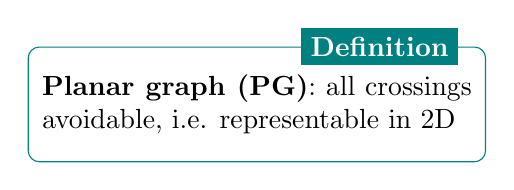
\begin{tikzpicture}
\node [rounded-box] (box){\begin{minipage}{0.45\textwidth}
    \textbf{Planar graph (PG)}: all crossings avoidable, i.e. representable in 2D
\end{minipage}};
\node[rounded-box-title, left=10pt] at (box.north east) {Definition};
\end{tikzpicture}

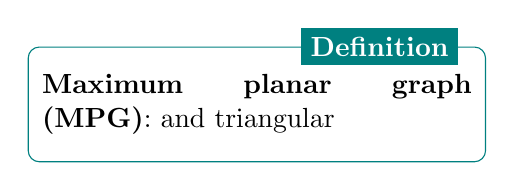
\begin{tikzpicture}
\node [rounded-box] (box){\begin{minipage}{0.45\textwidth}
    \textbf{Maximum planar graph (MPG)}: and triangular
\end{minipage}};
\node[rounded-box-title, left=10pt] at (box.north east) {Definition};
\end{tikzpicture}

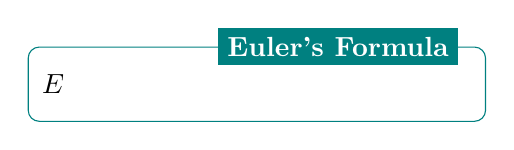
\begin{tikzpicture}
\node [rounded-box] (box){\begin{minipage}{0.45\textwidth}
    $E$
\end{minipage}};
\node[rounded-box-title, left=10pt] at (box.north east) {Euler's Formula};
\end{tikzpicture}

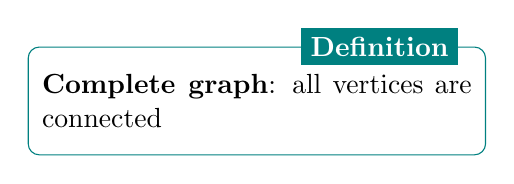
\begin{tikzpicture}
\node [rounded-box] (box){\begin{minipage}{0.45\textwidth}
    \textbf{Complete graph}: all vertices are connected
\end{minipage}};
\node[rounded-box-title, left=10pt] at (box.north east) {Definition};
\end{tikzpicture}

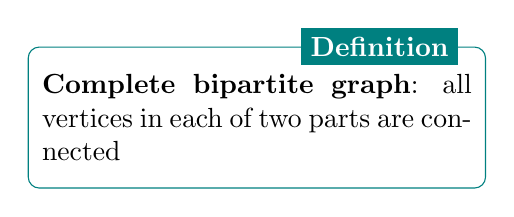
\begin{tikzpicture}
\node [rounded-box] (box){\begin{minipage}{0.45\textwidth}
    \textbf{Complete bipartite graph}: all vertices in each of two parts are connected
\end{minipage}};
\node[rounded-box-title, left=10pt] at (box.north east) {Definition};
\end{tikzpicture}

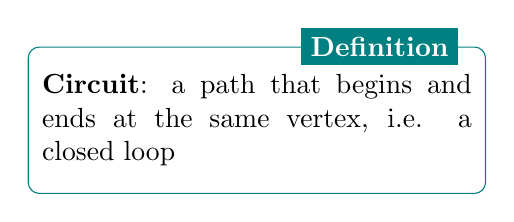
\begin{tikzpicture}
\node [rounded-box] (box){\begin{minipage}{0.45\textwidth}
    \textbf{Circuit}: a path that begins and ends at the same vertex, i.e. a closed loop
\end{minipage}};
\node[rounded-box-title, left=10pt] at (box.north east) {Definition};
\end{tikzpicture}

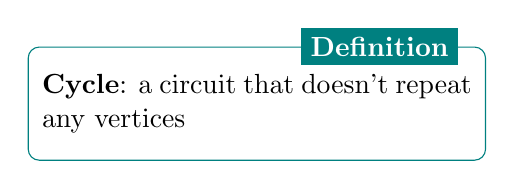
\begin{tikzpicture}
\node [rounded-box] (box){\begin{minipage}{0.45\textwidth}
    \textbf{Cycle}: a circuit that doesn't repeat any vertices
\end{minipage}};
\node[rounded-box-title, left=10pt] at (box.north east) {Definition};
\end{tikzpicture}

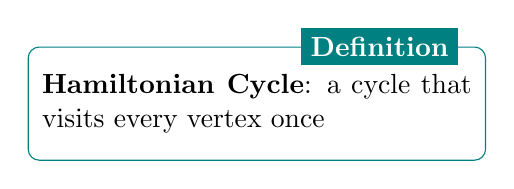
\begin{tikzpicture}
\node [rounded-box] (box){\begin{minipage}{0.45\textwidth}
    \textbf{Hamiltonian Cycle}: a cycle that visits every vertex once
\end{minipage}};
\node[rounded-box-title, left=10pt] at (box.north east) {Definition};
\end{tikzpicture}

Many (but not all) MPGs have a HC.

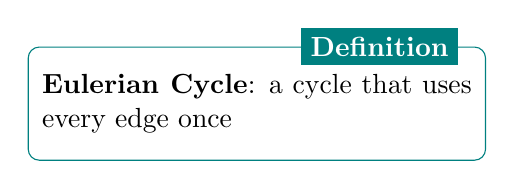
\begin{tikzpicture}
\node [rounded-box] (box){\begin{minipage}{0.45\textwidth}
    \textbf{Eulerian Cycle}: a cycle that uses every edge once
\end{minipage}};
\node[rounded-box-title, left=10pt] at (box.north east) {Definition};
\end{tikzpicture}

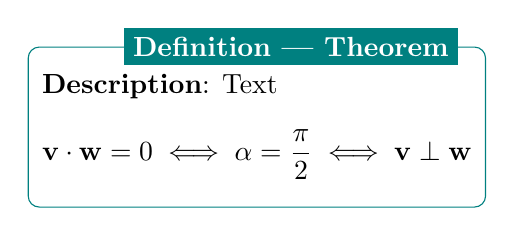
\begin{tikzpicture}
\node [rounded-box] (box){\begin{minipage}{0.45\textwidth}
    \textbf{Description}: Text
    $$\mathbf{v} \cdot \mathbf{w} = 0 \iff \alpha = \frac{\pi}{2} \iff \mathbf{v} \perp \mathbf{w}$$
\end{minipage}};
\node[rounded-box-title, left=10pt] at (box.north east) {Definition | Theorem};
\end{tikzpicture}

\end{paracol}
 \newpage
\input{section-5-connectivity-trees-cycles} \newpage
\section{Eulerian and Hamiltonian Cycles}

\subsection{Subsection 1}

\begin{paracol}{2}

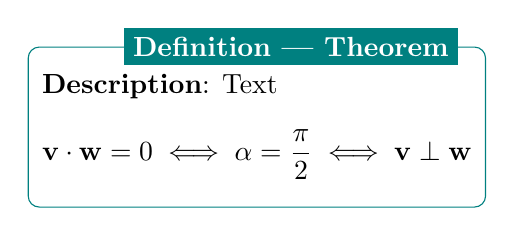
\begin{tikzpicture}
\node [rounded-box] (box){\begin{minipage}{0.45\textwidth}
    \textbf{Description}: Text
    $$\mathbf{v} \cdot \mathbf{w} = 0 \iff \alpha = \frac{\pi}{2} \iff \mathbf{v} \perp \mathbf{w}$$
\end{minipage}};
\node[rounded-box-title, left=10pt] at (box.north east) {Definition | Theorem};
\end{tikzpicture}

\end{paracol}
 \newpage
\input{section-7-spanning-trees} \newpage
\input{section-8-max-flow-min-cut} \newpage
\input{section-9-matchings-in-bipartite-graphs} \newpage

\nocite{*}
\printbibliography

\end{document}
